\documentclass[a4paper]{scrartcl}
\usepackage[english]{babel}
\usepackage[top=2cm,bottom=3cm,left=2.5cm,right=2.5cm]{geometry}
\usepackage[colorlinks=true, allcolors=black]{hyperref}
\usepackage{wrapfig} %문단 내 이미지 삽입
\usepackage{graphicx} %색상
\usepackage{overpic}
\usepackage[normalem]{ulem}%취소선
\usepackage{array} %표
\usepackage{mdframed, tcolorbox} %글상자
\usepackage[yyyymmdd]{datetime}
	\renewcommand{\dateseparator}{--}
\usepackage{amsmath, amsfonts, amssymb, bm} %수식
	\DeclareMathOperator{\arccsc}{arccsc}
	\DeclareMathOperator{\arcsec}{arcsec}
	\DeclareMathOperator{\arccot}{arccot}
	\DeclareMathOperator{\csch}{csch}
	\DeclareMathOperator{\sech}{sech}
	\DeclareMathOperator{\arcsinh}{arcsinh}
	\DeclareMathOperator{\arccosh}{arccosh}
	\DeclareMathOperator{\arctanh}{arctanh}
	\DeclareMathOperator{\arccsch}{arccsch}
	\DeclareMathOperator{\arcsech}{arcsech}
	\DeclareMathOperator{\arccoth}{arccoth}
	
	\DeclareMathOperator{\meter}{m}
	\DeclareMathOperator{\cm}{cm}
	\DeclareMathOperator{\mm}{mm}
	\DeclareMathOperator{\mum}{\mu m}
	\DeclareMathOperator{\newton}{N}
	\DeclareMathOperator{\kn}{kN}
	\DeclareMathOperator{\kgf}{kgf}
	\DeclareMathOperator{\pa}{Pa}
	\DeclareMathOperator{\kpa}{kPa}
	\DeclareMathOperator{\mpa}{MPa}
	\DeclareMathOperator{\gpa}{GPa}
	\DeclareMathOperator{\knpm}{kN/m}
	\DeclareMathOperator{\kph}{km/h}
	\DeclareMathOperator{\mps}{m/s}
	\DeclareMathOperator{\tkph}{kph}
	\DeclareMathOperator{\tmps}{mps}
	\DeclareMathOperator{\mpss}{m/s^2}
	\DeclareMathOperator{\dgr}{\!^\circ}
	\DeclareMathOperator{\cel}{\!^\circ C}
	\DeclareMathOperator{\kg}{kg}
	\DeclareMathOperator{\kgpcm}{kg/m^3}
	\DeclareMathOperator{\nm}{N\cdot m}
	\DeclareMathOperator{\knm}{kN\cdot m}
	\DeclareMathOperator{\kw}{kW}
	\DeclareMathOperator{\kwh}{kWh}
	\DeclareMathOperator{\mmhg}{mmHg}
	\DeclareMathOperator{\snd}{s}
\usepackage{polynom} %나눗셈 필산
\usepackage{cancel} %수식 약분선
\usepackage{titlesec} %섹션 이름 변경
	\titlespacing*{\section}{3mm}{0mm}{1mm}
	\titleformat{\section}{\bfseries\large}{}{0ex}{}
\usepackage{kotex} %한글

\newcommand{\prob}[2]{\section{#1}\begin{mdframed}#2\end{mdframed}}

\newlength{\picwidth}
\newcommand{\probpic}[4]{
	\setlength{\picwidth}{145mm}\addtolength{\picwidth}{-#3}\section{#1}\begin{mdframed}\begin{tabular}{m{#3}m{\picwidth}}
	\includegraphics[width = #3]{#2} & #4\end{tabular}\end{mdframed}
	}
	
\newcommand{\asw}[2]{
	\begin{flushright}
		#1\quad#2\quad$\blacktriangleleft$
	\end{flushright}
	}

\title{\vspace{100pt}\Huge{해설}}
\author{
	구조역학(박성훈 교수님) 2025-2 중간고사\\[10pt]
	시험 실시 : 2025-10-20 16:30-19:00(150분)\\[100pt]
	오류제보 : eunsoohong03@soongsil.ac.kr\\
	}
\date{\today}

\begin{document}

\renewcommand*{\titlepagestyle}{empty}
\maketitle

\vspace{60pt}

\begin{center}
	\includegraphics[width=0.45\textwidth]{SSU symbol KR-EN.jpg}
\end{center}

\newpage\setcounter{page}{1}

\probpic{Question 1 | Prob. 7.63}{img/q1.png}{40mm}{For the state of stress shown, it is known that the normal and shearing stresses are directed as shown and that $\sigma_x = 98\mpa$, $\sigma_y = 63\mpa$, and $\sigma_\text{min} = 35\mpa$. Determine ($a$) the orientation of the principal planes, ($b$) the principal stress $\sigma_\text{max}$, ($c$) the maximum in-plane shearing stress.}
	\begin{tabular}{m{55mm}m{105mm}}
		\includegraphics{img/q1-1.png} &
		$c = \cfrac{\sigma_x + \sigma_y}{2} = \cfrac{98+63}{2}\mpa = 80.5\mpa$\newline\newline
		$R = \sqrt{(\sigma_x - c)^2 + \tau_{xy}^2}$\newline
		$\sigma_\text{min} = c - R = c - \sqrt{(\sigma_x - c)^2 + \tau_{xy}^2}$\newline
		$(\sigma_x - c)^2 + \tau_{xy}^2 = (c - \sigma_\text{min})^2$
	\end{tabular}
	\begin{align*}
		&\tau_{xy}^2 = (c - \sigma_\text{min})^2 -(\sigma_x - c)^2\\
		&\tau_{xy}^2 = (\sigma_x - \sigma_\text{min})(2c - \sigma_\text{min} - \sigma_x)\\
		&\tau_{xy}^2 = (\sigma_x - \sigma_\text{min})(\sigma_y - \sigma_\text{min})\\
		&\tau_{xy} = \sqrt{(98-35)(63-35)}\mpa = 42\mpa\\
		&\theta_p = \frac{1}{2}\arctan\frac{\tau_{xy}}{\sigma_x - c} = \frac{1}{2}\arctan\frac{42}{98-80.5} = 33.69\dgr\quad\blacktriangleleft\quad(a)\\
		&R = \sqrt{(98 - 80.5)^2 + 42^2} = 45.5\mpa\\
		&\sigma_\text{max} = c + R = 126.00\mpa\quad\blacktriangleleft\quad(b)\\
		&\tau_\text{max} = R = 45.50\mpa\quad\blacktriangleleft\quad(c)
	\end{align*}

\newpage

\probpic{Question 2 | variation of 문제1 from HW2}{img/q2.png}{50mm}{A cantilever beam with a width $b = 100\mm$ and depth $h = 150\mm$ has a length $L = 2\meter$ and is subjected to a point load $P = 800\newton$ at $B$. Calculate the state of plane stress at point $C$ located $50\mm$ below the top of the beam and $0.5\meter$ to the right of point $A$. Also find the principal stresses and the maximum shear stress at $C$. Neglect the weight of the beam.}
	\begin{align*}
		&R_A = 800\newton\;(\uparrow),\quad M_A = (800\newton)(2\meter) = 1600\nm\;(\circlearrowleft)\\
		&\text{at $C$ :}\qquad V = 500\newton,\quad M = -1000\nm + (500\newton)(0.5\meter) = -1200\knm\\
		&I = \frac{bh^3}{12} = \frac{(0.1)(0.15)^3}{12}\meter^4 =  2.8125\times 10^{-5}\meter^4\\
		&\sigma_x = -\frac{My}{I} = -\frac{(-1200\nm)(0.05\meter)}{2.8125\times10^{-5}\meter^4} = \frac{3200}{3}\kpa = 1066.67\kpa
	\end{align*}
	\begin{tabular}{m{28mm}m{132mm}}
		\includegraphics{img/q2-1.png}
		&
		$Q = A\bar{y} = (0.1)(0.05)(0.05)\meter^3 = 2.5\times 10^{-4}\meter^3$\newline
		$\tau_{xy} = -\cfrac{VQ}{It} = -\cfrac{(800\newton)(2.5\times10^{-4}\meter^3)}{(2.8125\times 10^{-5}\meter^4)(0.1\meter)} = -\cfrac{640}{9}\kpa = -71.11\kpa$
	\end{tabular}
	\asw{$\sigma_x = 1066.67\kpa\;;\;\sigma_y =0\;;\;\tau_{xy} = -71.11\kpa$}{}
	\begin{tabular}{m{50mm}m{110mm}}
		\includegraphics{img/q2-2.png}
		&
		$c = \cfrac{\sigma_x}{2} =  \cfrac{1600}{3}\kpa$\newline\newline
		$R = \sqrt{c^2 + \tau_{xy}^2} = 538.0531893\kpa$\newline
		$\sigma_\text{max} = c + R = 1071.39\kpa$\newline
		$\sigma_\text{min} = c - R = -4.72\kpa$\newline
		$\tau_\text{max} = R = 538.05\kpa$
	\end{tabular}
	\asw{$\sigma_\text{max} = 1071.39\kpa\;;\;\sigma_\text{min} = -4.72\kpa\;;\;\tau_\text{max} = 538.05\kpa$}{}
	
\newpage

\probpic{Question 3 | Prob. 8.1}{img/q3.png}{45mm}{A W250$\times$101 rolled-steel beam supports a load $P$ as shown. Knowing that $P = 180\kn$, $a = 0.25\meter$, and $\sigma_\text{all} = 126\mpa$, determine ($a$) the maximum value of the normal stress $\sigma_m$, in the beam, ($b$) the maximum value of the principal stress $\sigma_\text{max}$ at the junction of the flange and web, ($c$) whether the specified shape is acceptable as far as these two stresses are concerned.(이유를 자세히 쓸 것)\newline\newline *Appendix E를 참고할 것}
	\begin{align*}
		&R_A = R_D = P = 180\kn\;(\uparrow)
	\end{align*}
	\includegraphics{img/q3-1.png}\\
	$M_\text{max} = (180\kn)(0.25\meter) = 45\knm$\\[10pt]
	\begin{tabular}{m{60mm}m{100mm}}
		\includegraphics{img/q3-2.png}
		&
		$c = \cfrac{d}{2} = 132\mm$\newline
		$y_j = c - t_f = (132 - 19.6)\mm = 112.4\mm$\newline
		$A = t_f b_f = (257)(19.6)\mm^2 = 5037.2\mm^2$\newline
		$I = 164\times10^6\mm^4 = 164\times10^{-6}\meter^4$\newline
		$\bar{y} = c - \cfrac{t_f}{2} = \left(132 - \cfrac{19.6}{2}\right)\mm = 122.2\mm$\newline
		$Q = A\bar{y} = (5037.2)(122.2)\mm^3 = 6.1554584\times10^{-4}\meter^3$
	\end{tabular}
	\begin{align*}
		&\sigma_m = \frac{M_\text{max}c}{I} = \frac{(45\times10^3)(0.132)}{164\times10^{-6}}\pa = 36.22\mpa\quad\blacktriangleleft\quad(a)\\
		&\sigma_x = - \frac{M_\text{max}y_j}{I} = - \frac{(45\times10^3)(0.1124)}{164\times10^{-6}}\pa = -\frac{2529}{82}\mpa = -30.84146341\mpa\\
		&\tau_{xy} = -\frac{VQ}{It_w} =  -\frac{(180\times10^3)(6.1554584\times10^{-4})}{(164\times10^{-6})(0.0119)}\pa = -56.773033\mpa\\
	\end{align*}
	\begin{tabular}{m{60mm}m{100mm}}
		\includegraphics{img/q3-3.png}
		&
		$c = \cfrac{\sigma_x}{2}$\newline
		$R = \sqrt{c^2 + \tau_{xy}^2}$\newline
		$\sigma_\text{max} = |c-R| = 74.25\mpa\quad\blacktriangleleft\quad(b)$\newline
		$\sigma_m < \sigma_\text{max} < \sigma_\text{all} \quad\Rightarrow\quad\text{Acceptable.}\quad\blacktriangleleft\quad(c)$
	\end{tabular}

\newpage

\probpic{Question 4 | Prob. 9.68}{img/q4.png}{60mm}{For the cantilever beam and loading shown, determine
	the slope and deflection at the free end.}
	In the case (1), $x$ is zero at the free end.\\
	\begin{tabular}{m{52mm}m{108mm}}
		\includegraphics[width = 48mm]{img/q4-1.png}
		&
		$M_1(x) = Pa = \text{const.}$\newline
		$EI\theta_1(x) = Pax + c_1,\quad \theta(L) = 0 \quad\Rightarrow\quad c_1 = -PaL$
	\end{tabular}
	\begin{align*}
		&EIy_1(x) = \cfrac{Pa}{2}x^2 - PaLx + c_2,\quad y(L) = 0 \quad\Rightarrow\quad c_2 = \cfrac{PaL^2}{2}\\
		&\theta_1(0) = \frac{c_1}{EI} = -\frac{PaL}{EI},\quad y_1(0) = \frac{c_2}{EI} = \frac{PaL^2}{2EI}
	\end{align*}
	In the case (2), $x$ is zero at point $B$ and the functions $\theta_2(x)$ and $y_2(x)$ are undefined at portion $AB$.\\
	\begin{tabular}{m{46mm}m{114mm}}
		\includegraphics[width = 42mm]{img/q4-2.png}
		&
		$V_2(x) = -P = \text{const.}$\newline
		$M_2(x) = -Px\quad(\because M(0) = 0)$\newline
		$EI\theta_2(x) = -\cfrac{P}{2}x^2 + c_1^*,\quad \theta_2(a) = 0 \quad\Rightarrow\quad c_1^* = \cfrac{Pa^2}{2}$
	\end{tabular}
	\begin{align*}
		&EIy_2(x) = -\frac{P}{6}x^3 +\frac{Pa^2}{2}x + c_2^*,\quad y_2(a) = 0 \quad\Rightarrow\quad c_2^* = -\cfrac{Pa^3}{3}\\
		&\theta_2(0) = \frac{c_1^*}{EI} = \frac{Pa^2}{2EI},\quad y_2(0) = \frac{c_2^*}{EI} = -\frac{Pa^3}{3EI}
	\end{align*}
	Superposition...
	\begin{align*}
		\theta_A
		&= \theta_1(0) + \theta_2(0) = \frac{Pa}{2EI}(a - 2L)\quad\blacktriangleleft\quad(\text{slope})\\
		y_A
		&= y_1(0) + y_2(0) + \theta_2(0)\times(a-L) = \frac{PaL^2}{2EI} - \frac{Pa^3}{3EI} + \frac{Pa^2}{2EI}(a-L)\\
		&= \frac{Pa}{6EI}\left\{3L^2 - 2a^2 + 3a(a-L)\right\} = \frac{Pa}{6EI}(a^2 - 3aL + 3L^2)\quad\blacktriangleleft\quad(\text{deflection})
	\end{align*}
	
\newpage

\probpic{Question 5 | variation of CA 9.5}{img/q5.png}{60mm}{For the loding shown, determine ($a$) the reaction force at $A$($R_A$), ($b$) equation of the elastic curve, ($c$) slope at $A$.}
	It's a statically indeterminate beam.
	\begin{align*}
		&+\uparrow\sum F_y = R_A + R_B - wL = 0,\quad R_A + R_B = wL\quad\cdots\quad(1)\\
		&+\circlearrowleft\sum M|_A = -wL\cdot\frac{L}{2} + R_BL + M_B = 0\quad\cdots\quad\text{We don't use this equation.}\\
		&M(x) = -wx\cdot\frac{x}{2} + R_Ax = -\frac{w}{2}x^2 + R_Ax\\
		&EI\theta(x) = -\frac{w}{6}x^3 + \frac{R_A}{2}x^2 + c_1,\quad \theta(L) = 0\quad\Rightarrow\quad \frac{R_AL^2}{2} + c_1 = \frac{wL^3}{6}\quad\cdots\quad(2)\\
		&EIy(x) = -\frac{w}{24}x^4 + \frac{R_A}{6}x^3 + c_1x + c_2,\quad y(0) = 0\quad\Rightarrow\quad c_2 = 0\\
		&y(L) = 0\quad\Rightarrow\quad \frac{R_AL^3}{6} + c_1L = \frac{wL^4}{24}\quad\cdots\quad(3)
	\end{align*}
	With equation (1), (2) and (3),
	\begin{align*}
		&\left(\begin{array}{ccc}
			1 & 1 & 0\\[5pt]
			\frac{L^2}{2} & 0 & 1\\[5pt]
			\frac{L^3}{6} & 0 & L
		\end{array}\right)
		\left(\begin{array}{c}
			R_A \\[5pt] R_B \\[5pt] c_1
		\end{array}\right)
		=
		\left(\begin{array}{c}
			wL \\[5pt] \frac{wL^3}{6} \\[5pt] \frac{wL^4}{24}
		\end{array}\right)\\
		&\Rightarrow\quad R_A = \frac{3}{8}wL\;(\uparrow)\quad\blacktriangleleft\quad(a)\quad,\quad R_B = \frac{5}{8}wL,\quad c_1 = -\frac{wL^3}{48}\\
		&EIy(x) = -\frac{w}{24}x^4 + \frac{wL}{16}x^2 - \frac{wL^3}{48}x\\
		&y(x) = -\frac{w}{48EI}(2x^4 - 3Lx^2 +L^3x)\quad\blacktriangleleft\quad(b)\\
		&\theta(0) = \frac{c_1}{EI} = -\frac{wL^3}{48EI}\quad\blacktriangleleft\quad(c)
	\end{align*}
	
	
\end{document}